\section{Test cases}
\subsection{Game-Explorer}

\begin{tabular}{cll}
	\hline
	\textbf{Test} & \textbf{Description} & \textbf{Tested Functionalities} \\
	\hline
	\ref{T:010} & \ref{T:010T} & \ref{FR:GE010}, \ref{FR:GE020} \\
	\ref{T:020} & \ref{T:020T} & \ref{FR:GE050} \\
	\ref{T:030} & \ref{T:030T} & \ref{FR:GE030} \\
	\ref{T:040} & \ref{T:040T} & \ref{FR:GE040} \\
	\hline
\end{tabular}

\begin{description}
	\item[\textlabel{/T010/}{T:010}] \textbf{\textlabel{Start the Game-Explorer}{T:010T}} \\
	\textbf{Input:} The tester clicks the Game-Explorer icon. \\
	\textbf{Exp. Output:} The Game-Explorer window opens, the game folder is scanned and all games contained are shown in the games list.
	
	\item[\textlabel{/T020/}{T:020}] \textbf{\textlabel{Select a game}{T:020T}} \\
	\textbf{Input:} The tester clicks on the name of the game in the list. \\
	\textbf{Exp. Output:} An image and a description of the game are displayed.
	
	\item[\textlabel{/T030/}{T:030}] \textbf{\textlabel{Start a game}{T:030T}} \\
	\textbf{Input:} A game has been selected and the tester clicks on the start button. \\
	\textbf{Exp. Output:} The game window opens.
	
	\item[\textlabel{/T040/}{T:040}] \textbf{\textlabel{Use the help function}{T:040T}} \\
	\textbf{Input:} A game has been selected and the tester clicks on the help button. \\
	\textbf{Exp. Output:} The help page is displayed in a new window.
\end{description}

\subsection{Games}
\subsubsection\graphcoloring

\begin{tabular}{cll}
	\hline
	\textbf{Test} & \textbf{Description} & \textbf{Tested Functionalities} \\
	\hline
	\ref{T:050} & \ref{T:050T} & \ref{FR:L010}, \ref{FR:L020},\ref{FR:GU010}, \\
	 & & \ref{FR:GU020} \\
	\ref{T:060} & \ref{T:060T} & \ref{FR:G010}, \ref{FR:G020}\\
	\ref{T:070} & \ref{T:070T} & \ref{FR:L040}, \ref{FR:L050}, \ref{FR:GU030} \\
	\ref{T:080} & \ref{T:080T} & \ref{FR:L040}, \ref{FR:L050}, \ref{FR:GU030}\\
	\ref{T:090} & \ref{T:090T} & \ref{FR:L040}, \ref{FR:L050}, \ref{FR:L100}, \\
	 & & \ref{FR:GU030}, \ref{FR:GU040}\\
	\ref{T:100} & \ref{T:100T} & \ref{FR:L100}, \ref{FR:GU040} \\
	\ref{T:110} & \ref{T:110T} & \ref{FR:L100}, \ref{FR:GU040} \\
	\hline
\end{tabular}



\begin{description}
	\item[\textlabel{/T050/}{T:050}] \textbf{\textlabel{Start the game}{T:050T}} \\
	\textbf{Input:} \graphcoloring has been selected and the tester clicks on the start button. \\
	\textbf{Exp. Output:} The game window opens and the graph of the first level is displayed.
	
	\item[\textlabel{/T060/}{T:060}] \textbf{\textlabel{Save and load a game}{T:060T}} \\
	\textbf{Input:} Some vertices have been colored. The tester saves the current state, closes and reopens \graphcoloring and loads the savegame. \\
	\textbf{Exp. Output:} The state is saved in a file and when the file is loaded, the saved state is restored.
	
	\item[\textlabel{/T070/}{T:070}] \textbf{\textlabel{Color an uncolored vertex}{T:070T}} \\
	\textbf{Input:} The tester selects a color and clicks on an uncolored vertex that is not adjacent to one in the same color. \\
	\textbf{Exp. Output:} The vertex changes its color to the selected one.
	
	\item[\textlabel{/T080/}{T:080}] \textbf{\textlabel{Color a colored vertex}{T:080T}} \\
	\textbf{Input:} The tester selects a color and clicks on a colored vertex. \\
	\textbf{Exp. Output:} Nothing changes.
	
	\item[\textlabel{/T090/}{T:090}] \textbf{\textlabel{Color adjacent vertices in the same color}{T:090T}} \\
	\textbf{Input:} The tester selects a color and clicks on an uncolored vertex that is adjacent to one in the same color. \\
	\textbf{Exp. Output:} The vertex does not change. An error message is displayed.
	
	\item[\textlabel{/T100/}{T:100}] \textbf{\textlabel{Win/Lose a single-player game}{T:100T}} \\
	\textbf{Input:} The tester plays until he won/lost the game. \\
	\textbf{Exp. Output:} A win/lose message is displayed and the next/same level is loaded.

	\item[\textlabel{/T110/}{T:110}] \textbf{\textlabel{Win/Lose a multiplayer game}{T:110T}} \\
	\textbf{Input:} The tester plays for both players until one won the game. \\
	\textbf{Exp. Output:} A win message for the winning player is displayed.
	
\end{description}

\subsubsection\twixt

\begin{tabular}{cll}

\hline
	\textbf{Test} & \textbf{Description} & \textbf{Tested Functionalities} \\
	\hline
	\ref{T:120} & \ref{T:120T} & \ref{FR:L010}, \ref{FR:L020},\ref{FR:GU010} \\
	\ref{T:130} & \ref{T:130T} & \ref{FR:G010}, \ref{FR:G020} \\
	\ref{T:140} & \ref{T:140T} & \ref{FR:L030}, \ref{FR:L040}, \ref{FR:L100}, \\
	 & & \ref{FR:GU040} \\
	\ref{T:150} & \ref{T:150T} & \ref{FR:L030}, \ref{FR:L040}, \ref{FR:L080}, \\
	 & & \ref{FR:L100},  \ref{FR:GU040} \\
	\ref{T:160} & \ref{T:160T} & \ref{FR:L030}, \ref{FR:L040}, \ref{FR:L100}, \\
	 & & \ref{FR:GU040} \\
	\ref{T:170} & \ref{T:170T} & \ref{FR:L030}, \ref{FR:L040} \\
	\ref{T:180} & \ref{T:180T} & \ref{FR:L060}, \ref{FR:L070} , \ref{FR:L100}, \\
	& & \ref{FR:GU040} \\
	\hline
\end{tabular}

\begin{description}
	\item[\textlabel{/T120/}{T:120}] \textbf{\textlabel{Start the game}{T:120T}} \\
	\textbf{Input:} \twixt has been selected and the tester clicks on the start button. \\
	\textbf{Exp. Output:} The game window opens and the empty grid is displayed.
	
	\item[\textlabel{/T130/}{T:130}] \textbf{\textlabel{Save and load a game}{T:130T}} \\
	\textbf{Input:} Some vertices have been placed. The tester saves the current state, closes and reopens \twixt and loads the savegame. \\
	\textbf{Exp. Output:} The state is saved in a file and when the file is loaded, the saved state is restored.
	
	\item[\textlabel{/T140/}{T:140}] \textbf{\textlabel{Place edges and vertices}{T:140T}} \\
	\textbf{Input:} The tester places vertices and connects them with edges for both players without intersection. \\
	\textbf{Exp. Output:} The placed vertices and edges are displayed. Each turn the status displays which player's turn it is.
	
	\item[\textlabel{/T150/}{T:150}] \textbf{\textlabel{Place an edge across another one}{T:150T}} \\
	\textbf{Input:} Two vertices have been connected by an edge. The tester clicks on two other vertices on either side of the edge. \\
	\textbf{Exp. Output:} The vertices do not get connected. An error message is displayed.
	
	\item[\textlabel{/T160/}{T:160}] \textbf{\textlabel{Connect vertices of wrong distance}{T:160T}} \\
	\textbf{Input:} Two vertices have been placed that are not in a knight's move distance. The tester clicks them both. \\
	\textbf{Exp. Output:} The vertices do not get connected. An error message is displayed.
	
	\item[\textlabel{/T170/}{T:170}] \textbf{\textlabel{Place a vertex on an already occupied field}{T:170T}} \\
	\textbf{Input:} A vertex has been placed. The tester clicks the vertex again. \\
	\textbf{Exp. Output:} Nothing changes.
	
	\item[\textlabel{/T180/}{T:180}] \textbf{\textlabel{Win/Lose a game}{T:180T}} \\
	\textbf{Input:} The tester plays for both players until one won the game. \\
	\textbf{Exp. Output:} A win message for the winning player is displayed.
\end{description}

\subsection{Test scenarios}

\subsubsection{Use the Game-Explorer}

Alice starts the Game-Explorer and selects \graphcoloring in the list in order to look at the screenshot and the description of the game. Still not convinced, Alice uses the help function to gain an insight in how \graphcoloring works. Then Alice starts the game.

\subsubsection{Play \graphcoloring single-player} \label{T:GCSingle}

Bob starts \graphcoloring with the Game-Explorer. Bob selects the color red and colors vertex 1. Then Bob selects blue, colors vertex 3 and 4 and tries to color vertex 2, but it stays uncolored. The status bar displays an error message for a few seconds. Bob then selects green and colors vertex 2. A win message is displayed. Then Bob closes the game.

\subsubsection{Play \graphcoloring multiplayer} \label{T:GCMulti}

Carol and Dave start \graphcoloring with the Game-Explorer. Carol selects the color blue and colors vertex 2. Dave selects red and colors vertex 4. Carol selects green and tries to color vertex 2, but it stays blue. Carol then colors vertex 3. Since no valid move is possible anymore, a win message for Carol is displayed. Dave then closes the game.

\begin{figure}[h!]
	\centering
	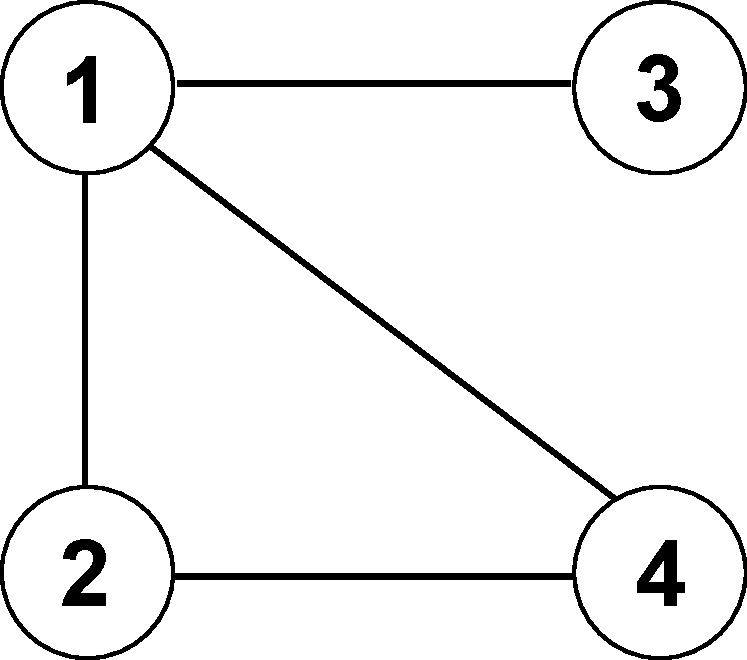
\includegraphics[width=0.25\textwidth]{testgraph.pdf}
	\caption{Graph the scenarios \ref{T:GCSingle} and \ref{T:GCMulti} are based on}
	\label{img:ACTDEV}
\end{figure}

\subsubsection{Play \twixt} \label{T:TwixT}

Carol and Dave start \twixt with the Game-Explorer. They select a 7$\times$7 grid and the grid is displayed. Dave starts and places a vertex on position C3. Carol places a vertex on position E3. Dave places a vertex on position E4. Carol places a vertex on position D5. Dave connects his placed vertices with an edge. Carol also tries to connect the vertices she placed. The status bar displays an error message for a few seconds. Carol then places a vertex on position F5. Dave connects the vertex on C3 with the vertex of his left border row on position A4. Carol tries to place a vertex on position C3, but it does not change. Carol then connects the vertex on E3 with her upper border row on position F1. Dave closes his path by connecting his vertex on E4 with his right border row on position G3. A win message for Dave is displayed. Dave then closes the game.

\begin{figure}[h!]
	\centering
	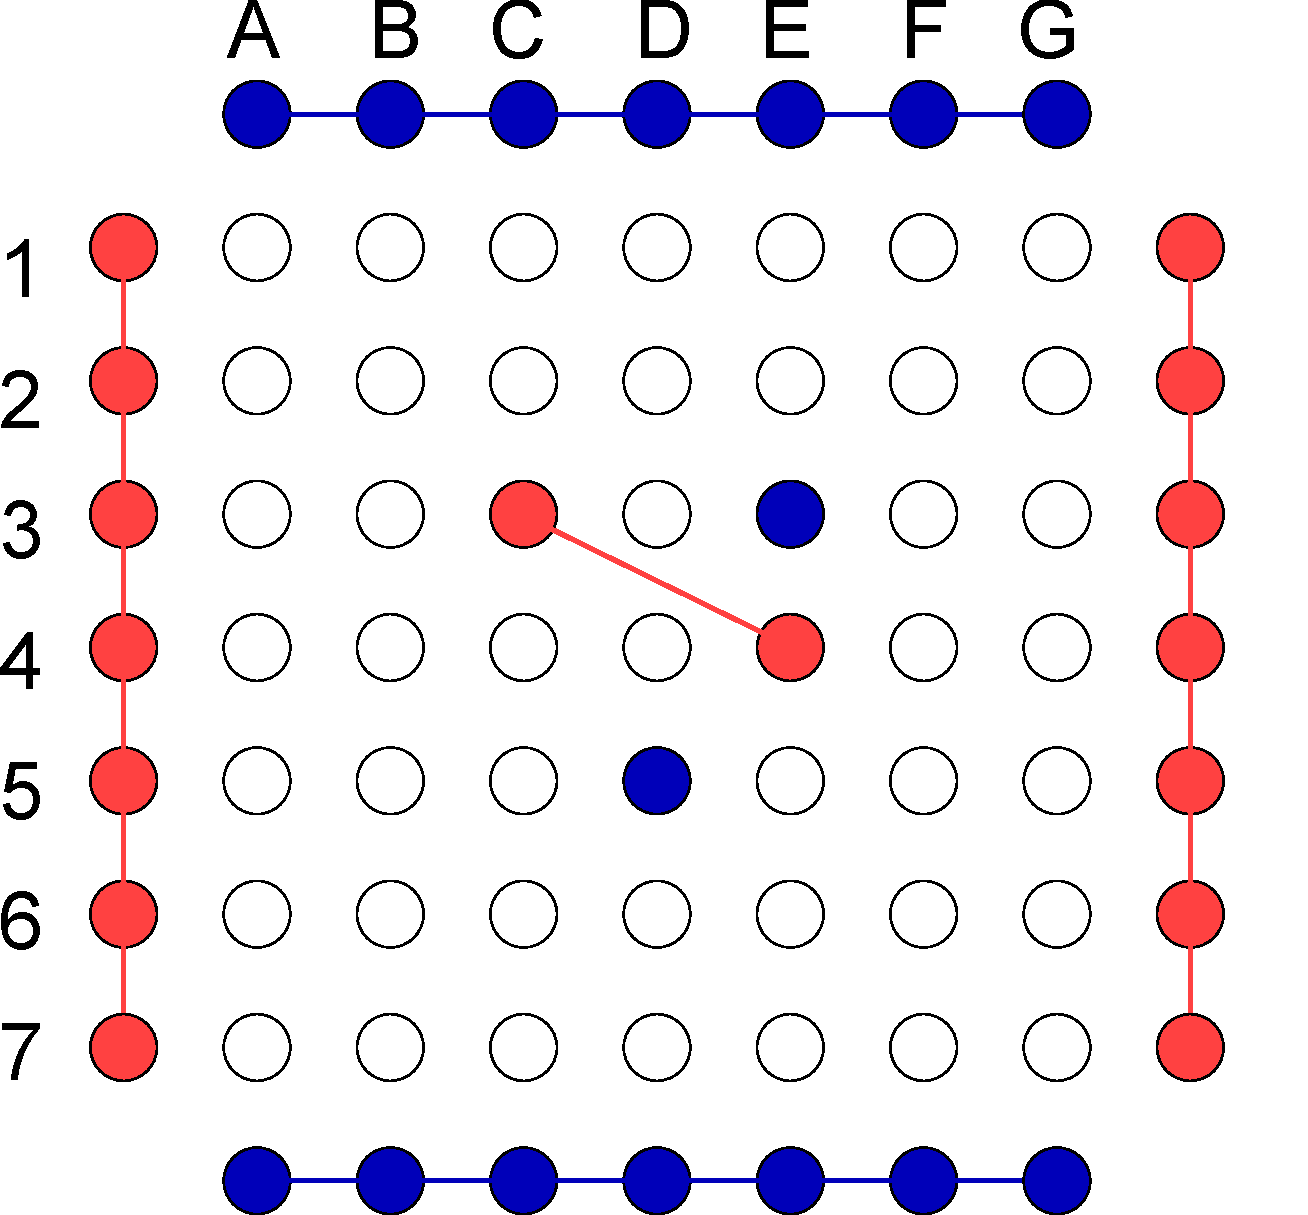
\includegraphics[width=0.35\textwidth]{testtwixt.pdf}
	\caption{Scenario \ref{T:TwixT} after Dave's (red) third move}
	\label{img:ACTDEV}
\end{figure}